%-----------------------------------------------------------------------------
%
%               Template for sigplanconf LaTeX Class
%
% Name:         sigplanconf-template.tex
%
% Purpose:      A template for sigplanconf.cls, which is a LaTeX 2e class
%               file for SIGPLAN conference proceedings.
%
% Guide:        Refer to "Author's Guide to the ACM SIGPLAN Class,"
%               sigplanconf-guide.pdf
%
% Author:       Paul C. Anagnostopoulos
%               Windfall Software
%               978 371-2316
%               paul@windfall.com
%
% Created:      15 February 2005
%
%-----------------------------------------------------------------------------


\documentclass{sigplanconf}

% The following \documentclass options may be useful:

% preprint      Remove this option only once the paper is in final form.
% 10pt          To set in 10-point type instead of 9-point.
% 11pt          To set in 11-point type instead of 9-point.
% authoryear    To obtain author/year citation style instead of numeric.
\usepackage[utf8]{inputenc}
\usepackage{amsmath}
\usepackage{hyperref}
\usepackage{graphicx}
\usepackage{caption}
\usepackage{multirow}

\begin{document}

\special{papersize=8.5in,11in}
\setlength{\pdfpageheight}{\paperheight}
\setlength{\pdfpagewidth}{\paperwidth}

\conferenceinfo{CONF 'yy}{Month d--d, 20yy, City, ST, Country} 
\copyrightyear{20yy} 
\copyrightdata{978-1-nnnn-nnnn-n/yy/mm} 
\doi{nnnnnnn.nnnnnnn}

% Uncomment one of the following two, if you are not going for the 
% traditional copyright transfer agreement.

%\exclusivelicense                % ACM gets exclusive license to publish, 
                                  % you retain copyright

\permissiontopublish             % ACM gets nonexclusive license to publish
                                  % (paid open-access papers, 
                                  % short abstracts)

\titlebanner{banner above paper title}        % These are ignored unless
\preprintfooter{short description of paper}   % 'preprint' option specified.

\title{Uniforms}
\subtitle{e-Formulaire, Rapport Scientifique}

\authorinfo{Michel Gautero}
           {I3S}
           {Michel.Gautero@unice.fr}
\authorinfo{Ayoub Benathmane}
           {M2 IFI}
           {benathmane.ab@gmail.com}
\authorinfo{Genevi\`eve Cirera}
           {SI5}
           {genevieve.cirera@gmail.com}
\authorinfo{Lu\'is Felipe Polo}
           {SI5}
           {luisfelipepolo@hotmail.com}
\authorinfo{Romain Truchi}
           {M2 IFI}
           {romain.truchi.06@gmail.com}

\maketitle

\begin{abstract} %TODO
This is the text of the abstract.
\end{abstract}

\category{CR-number}{subcategory}{third-level}

% general terms are not compulsory anymore, 
% you may leave them out
\terms
term1, term2

\keywords
Uniforms, form

%-----------------------Section introduction
\section{Introduction}
De nos jours, deux types de formulaire existent. Les formulaires papiers, distribués puis collectés physiquement et les formulaires électroniques, qui peuvent être envoyés par e-mail, les destinataires répondent alors par l’intermédiaire d’une page web leur affichant les questions et les champs de réponses possibles.\\
L’idée générale de ce projet est de proposer une manière de concevoir les formulaires, les partager et les gérer sans avoir recours à une application externe à l’université Nice Sophia Antipolis car de nombreuses applications de création de formulaire existantes collectent et conservent les données sur leurs serveurs. Il faut également que notre application puisse proposer les deux types de transmission, physique, grâce à une fonctionnalité d’impression des formulaires, et électronique.\\
D’autres points sont essentiels à ce projet comme le besoin de proposer une interface intuitive à l’utilisateur, qu’il puisse comprendre facilement le fonctionnement de l’application et qu’il ne perde pas de temps, que l’application soit bénéfique tout autant dans le temps que par les possibilités de création et de gestion par rapport à ses moyens actuels. \\
De plus, l’application devra être compatible avec les technologies de l’université car elle y sera hébergée.\\

%TODO énoncer le plan correctement, Attention à ce que le plan annoncé corresponde effectivement au plan du rapport.
Nous verrons tout d'abord les scénarios issus des besoins de cette application, puis la description de notre contribution, les tests réalisés, le positionnement de notre application par rapport à l'état de l'art pour enfin conclure.


%------------------Section scénario
\section{Scénarios}\label{sec:scenarios}
Notre problème se décompose en plusieurs scénarios distincts, la création/modification de formulaire, la consultation des réponses, la réalisation des réponses à un formulaire non anonyme et anonyme et le remplissage de formulaire papier. Nous pouvons voir un résumé de tous ces scénarios figure~\ref{scenarios} avec leurs descriptifs figure~\ref{listScenarios}.
\begin{figure} %TODO mettre à jour l'image
\begin{center}
\makebox[\linewidth]{%        to center the image
  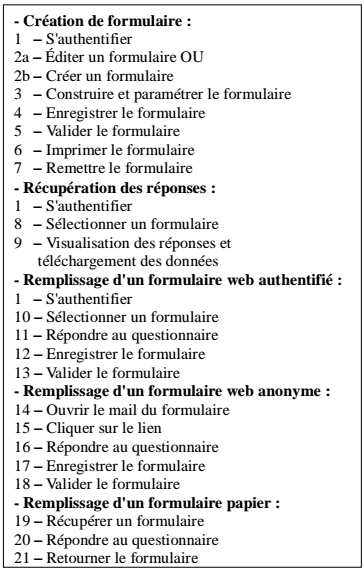
\includegraphics [width=70mm]{images/listScenarios.png}}
\end{center}
\caption{Descriptif des scénarios}
\label{listScenarios}
\end{figure}

\subsection{S'authentifier}
L’utilisateur doit tout d’abord s'identifier avec le CAS\footnote{Central Authentification Service} ou localement. Ce n'est qu'ensuite qu'il aura la possibilité de créer des formulaires ou de répondre à ceux qui lui ont été adressés.

\subsection{Créer un formulaire et le soumettre}
Une fois authentifié, l'utilisateur peut cliquer sur “Créer un formulaire”, une interface lui sera proposée afin qu’il puisse placer les éléments par glisser-déposer\footnote{Aussi connu sous le nom de drag and drop} là où il le souhaite. Les éléments sont divers, label pour écrire une question, des boutons radios ou cases à cocher pour une question à choix multiple...\\
Par défaut, tous les éléments sont dans un même groupe.\\
L’utilisateur peut ensuite définir les paramètres pour que le formulaire soit imprimable et/ou anonyme. Si ce dernier est anonyme alors il ne sera pas nécessaire de se connecter pour répondre à ce formulaire et les personnes pouvant répondre à ce formulaire sont celles disposant du lien.\\
Si le formulaire est imprimable alors les éléments seront arrangés de telle manière à ce qu’ils puissent être sur une page A4.\\
De plus, l’utilisateur peut définir le nombre de réponse accepté par personne pour un même formulaire, de 1 à l’infini.\\
Après ces paramétrages, l’utilisateur peut soit enregistrer, soit publier le formulaire. Dans ce dernier cas, le formulaire ne pourra plus être modifié et pourra être rempli par ses destinataires.\\

\begin{figure} %TODO mettre à jour l'image
\begin{center}
\makebox[\linewidth]{%        to center the image
  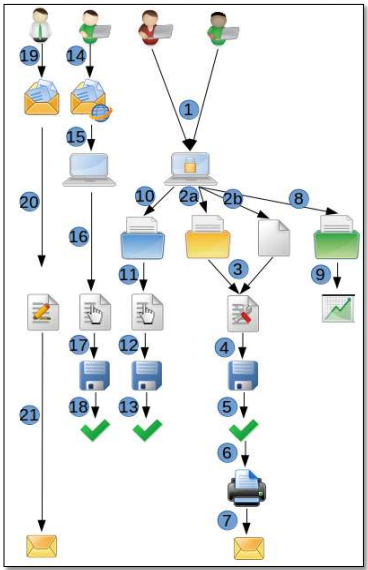
\includegraphics [width=70mm]{images/scenarios.png}}
\end{center}
\caption{Scénarios}
\label{scenarios}
\end{figure}

\subsection{Créer un formulaire avec des groupes}
Lors de la création d'un formulaire, l'utilisateur peut créer des groupes d'éléments pour que le formulaire soit répondu par un ensemble de personnes en assignant les groupes des champs à un ou plusieurs destinataires. C’est-à-dire que les personnes assignées à un groupe d’éléments seront les seules personnes autorisées à remplir ces champs là (cette fonctionnalité sera très utile si le formulaire est une demande d’autorisation et que la même personne doit donner son accord pour toutes les demandes).\\
Pour chaque groupe créé, l'utilisateur doit renseigner le ou les destinataires ainsi que le nombre de fois que le formulaire peut être répondu par chaque destinataire.\\
L'utilisateur peut ensuite enregistrer ou publier le formulaire. Si un champs est manquant, une alerte s'affichera.

\subsection{Modifier un formulaire}
Les formulaires enregistrés peuvent être modifiés. Parmi toute la liste des formulaires qu’il a créés, l’utilisateur peut modifier ceux qui ne sont pas publiés. Dans ce cas, la page de création de formulaire lui est présentée préremplie par les informations enregistrées du formulaire en cours de construction. 

\subsection{Consulter les réponses}
Le créateur peut consulter les réponses des formulaires qu’il a créés. Pour cela, il doit s’identifier sur la plate-forme, puis aller sur la page de consultation des réponses du formulaire souhaité. Les réponses réalisées par les destinataires sont affichées sans attendre que tous les destinataires aient répondu.\\
Les réponses peuvent être consultées directement sur l’application ou bien être téléchargées en CSV et/ou SQL\footnote{Structured Query Language}.

\subsection{Répondre à un formulaire}
Pour les formulaires non anonymes, les destinataires doivent tout d’abord s’identifier pour pouvoir y répondre. Ils accèdent ensuite à l’ensemble des formulaires dont ils sont destinataires et ils peuvent alors y répondre. \\
Une fois répondu, ils ont le choix entre enregistrer la réponse ou l'envoyer. “Enregistrer” permet de modifier la réponse plus tard, “Envoyer” envoie la réponse au créateur du formulaire, elle ne sera plus modifiable.\\
Pour les formulaires anonymes, aucune identification n’est obligatoire, les personnes possédant le lien du formulaire peuvent y répondre, en revanche enregistrer une réponse pour la modifier plus tard est impossible car anonyme, le formulaire doit être rempli en une seule fois.

\subsection{Soumission de formulaire papier}
Le créateur dispose d’une fonctionnalité d’impression du formulaire, il peut alors distribuer les formulaires en main propre et collecter les réponses physiquement. \\


%--------------------------Section technologie
%\section{Contribution}
\section{Choix des technologies}
Le choix des technologies s’est fait très rapidement en début de projet, nous avons décidé des langages, librairies, frameworks et outils de gestion de projet.
\subsection{Langages}
\subsubsection{Coté serveur}
Pour réaliser un site dynamique comme le notre, il est nécessaire d'utiliser un langage serveur.\\
Plusieurs langages sont disponibles, ASP\footnote{Active Server Pages} .NET, Ruby on Rails, Django, JEE\footnote{Java Enterprise Edition},... Tous ont leurs avantages et inconvénients.\\
ASP .NET exploite le framework .NET, est très proche du dévelop-pement en C\# et est propriétaire, Django au contraire est un framework Python open-source, JEE pour les développeurs Java...\\
Au niveau des services des frameworks, Django et Ruby on Rails sont en tête, cependant, les services proposés ne nous sont pas forcément nécessaires. Pour contruire une application web ``simple'' et n'ayant pas tous les mêmes compétences, PHP\footnote{Hypertext Preprocessor} nous a paru la meilleure option car, pour ceux d'entre nous ne connaissant aucun de ces langages, le temps d'apprentissage est relativement court ce qui permettrait un avancement plus rapide. De plus, nous ne perdons pas la possibilité d'exploiter l'orienté objet.\\

Pour la base de données, plusieurs SGBD\footnote{Système de Gestion de Base de Données} sont possibles, Oracle, PostgreSQL, MySQL, MongoDB...\\
Oracle est propriétaire, MongoDB est un SBGD NoSQL\footnote{Not only SQL}, PostgreSQL et MySQL quant à eux sont libre et relationnel.\\
Pour notre application, nous avions besoin d'un SGBDR\footnote{Système de Gestion de Base de Données Relationnelles}, MySQL et PostgreSQL paraissaient donc de bonnes options.\\

Nous avions également une contrainte de déploiement, l'application devait pouvoir être hébergée à l'UNS\footnote{Université Nice Sophia Antipolis}, PHP\cite{urlPHP} et MySQL\cite{urlMySQL} étaient donc les choix les plus sages.\\
Les versions utilisées sont les suivantes : 
\begin{description}
\item [PHP] : 5.4.* utilisé en orienté objet
\item [MySQL] : 5.5.*
\end{description}

\subsubsection{Coté client}\label{langagesClient}
Plusieurs langages sont nécessaires coté client, un langage de balisage (HTML\footnote{Hypertext Markup Language}, XML\footnote{eXtended Markup Language}, Latex,...), un langage de script (JavaScript, ActionScript, JScript, VBScript\footnote{Microsoft Visual Basic Scripting Edition},...) et des feuilles de style (CSS\footnote{Cascading Style Sheets}).
\begin{itemize}
\item Langage de balisage\\
Parmis tous les langages étudiés, HTML nous a paru le plus adapté car multiplateforme, tous les navigateurs le reconnaissent et est facile à mettre en place, peu de connaissances sont nécessaires.
\item Langage de script\\
JScript est une adaptation de JavaScript par Microsoft, VBScript a été développé par Microsoft et est un sous-ensemble de Visual Basic, il est donc propre à Microsoft.\\
JavaScript étant le langage le plus utilisé et étant reconnu par tous les navigateurs, nous avons décidé de l'utiliser.
\end{itemize}

De plus, la facilité et simplicité d'utilisation, la rapidité d'appren-tissage des langages et la contrainte de déploiement nous ont mené vers le choix de HTML, CSS et JavaScript.\\
Les versions utilisées sont les suivantes :
\begin{description}
\item [HTML5]
\item [CSS3]
\end{description}

Cependant, tout développer depuis zéro, nous paraissait trop long et fastidieux, de plus, javaScript peut avoir des résultats différents suivant les navigateurs, c'est pourquoi nous avons décidé d'utiliser des librairies et frameworks.

\subsection{Librairie/Framework}\label{librairieFramework}
Nous avons choisi JQuery\cite{urljQuery}, une librairie JavaScript libre, pour sa simplicité et efficacité afin de faciliter l'écriture de scripts coté client.\\
Certaines fonctionnalités comme le glisser-déposer est plus facile à implémenter depuis cette librairie qu’en JavaScript pur. JQuery propose de nombreuses fonctionnalités telles que le parcours et modification du DOM\footnote{Document Object Model}, gestion des événements, création d'effets visuels et d'animations,...\\
JQuery est une librairie relativement complète mais n'est pas un framework, ce qui veut dire que le développement de l'application ne sera pas ``enfermé'' et nous garderons une certaine liberté de développement.\\

En ce qui concerne le design, il nous paraissait difficile de créer toutes les feuilles de style, en définissant les couleurs, dispositions, formes,...de chaque élément. C'est pourquoi, nous avons choisi d’utiliser Bootstrap\cite{urlBootstrap}.\\
À la différence de ses concurrents (par exemple Foundation from Zurb) Bootstrap est plus simple d’utilisation, son apprentissage est rapide et il propose des styles prédéfinis sans besoin de configuration préalable.\\
Bootstrap nous a ainsi permis de réaliser une application responsive avec un style prédéfini Bootstrap sans trop de difficulté.\\
Les versions utilisées sont les suivantes :
\begin{description}
\item [JQuery] : 2.1.1
\item [Bootstrap] : 3.3.1
\end{description}

Il nous a fallu investir du temps d'apprentissage pour ces deux technologies, cependant, ce temps était nécessaire afin d'être plus efficace pour le reste du développement.

\subsection{Gestion de projet}
Pour la gestion de notre projet, deux outils principaux ont été utilisés. Un outil de gestion de version git avec un dépôt privé sous Github et un gestionnaire de tâches sur la plateforme JIRA.\\
Le gestionnaire de version nous permet de partager du code et de travailler collaborativement.\\
Le gestionnaire de tâches est un système de tickets, l’équipe en définit tout un ensemble et chaque membre réalise les tâches qui lui sont attribuées. Chaque membre place le ticket en zone “Progress” puis “Done” une fois terminée ainsi nous avons pu suivre l’avancée de chaque membre et éviter les conflits de merge avec le gestionnaire de version.\\
Les tâches ont été définies de telles manière à suivre la méthode agile décrite dans le DoW\footnote{Description Of Work} et pouvoir progresser en lot.

%------------------------Section management
\section{Management}
\subsection{Planning prévisionnel}
Les fonctionnalités à développer ont été séparer en tâches qui ont été regroupées en lot. Tous les lots ont été prévus pour certaines semaines voir tableau~\ref{planifPrev}.

\begin{table}
\begin{center}
\begin{tabular}{|c|p{5cm}|c|c|}
\hline
 \# & Titre du lot & Début & Fin \\ \hline
L1 & Management du projet & S1 & S21\tabularnewline
L2 & Cœur de l'application & S5 & S7\tabularnewline
L3 & Réponses Multiples & S7 & S7.5\tabularnewline
L4 & Eléments basiques + D\&D + CSV & S7.5 & S8\tabularnewline
L5 & Fonctionnalités de Création + Collaboration & S8 & S14\tabularnewline
L6 & CAS + BDD Ext + Destinataires (Test déploiement) & S14 & S18\tabularnewline
L7 & Eléments Avancés + CSV & S20 & S20\tabularnewline
L8 & Déploiement à l'Université & S20 & S20\tabularnewline
L9 & Présentation de l'application & S21 & S21\\
\hline
\end{tabular}
\end{center}
\caption{Planification prévisionnelle}\label{planifPrev}
\end{table}

\subsection{Reunions}
Au début du projet, nous avions plannifié une réunion après chaque fin de lot avec notre tuteur pour validation. Cependant, durant les périodes à temps partiels, tous les membres du group n'ont pas le même emploi du temps et notre tuteur non plus, un créneau disponible était difficil à trouver. C'est pourquoi, beaucoup de mail ont été échangés afin de compenser les réunions qui ne pouvaient pas avoir lieu.\\
Pour les démonstrations de l'application, à partir de février, nous avons réalisé un déploiement sur un serveur de test, l'application était donc accessible sur \url{http://uniform.gautero.fr/}. Ainsi, notre tuteur pouvait voir l'avancement ainsi que nous commenter les améliorations souhaitées et bugs rencontrés.

\subsection{Imprévus}
Après la réalisation du DoW, une nouvelle ressource a été disponible pour le projet, il a donc fallu revoir les fonctionnalités à développer, en ajouter et revoir la plannification. Un nouveau lot a donc été ajouté, la ``Collaboration'' qui consiste à rendre un formulaire remplissable par plusieurs personnes.\\
D'autre part, du retard a été pris durant le projet, dû à des développements qui ont pris plus de temps que prévu, les spécificités de la ``Collaboration'' ont été ajustées au fur et à mesure et sa conception et son développements à pris plus de temps. Il nous aura fallu plusieurs réunions avec le client pour mettre au point une solution adapté au besoin.\\
Les conséquences du retard de ce lot a été que le lot d'interfaçage avec base de données externes n'a pas été réalisé car les spécificités de ce lot ont aussi été ajusté, son développement demandait plus de temps que prévu également, c'est pourquoi avec l'accord du client, nous avons décidé de nous concentrer sur les autres fonctionnalités et d'abandonner le lot de l'interfaçage.\\
Par manque de temps, nous avons également décidé de ne développer qu'une partie des éléments pouvant être placés dans le formulaire. Les éléments ont été choisis de manière à ce qu'un maximum de possibilité soit proposer, par exemple, le champs URL peut être remplacé par un champs d'entrée simple.

\subsection{Planning réalisé}
Face aux imprévus, il nous a fallu adapter notre planification, notamment l'interfaçage avec la base de données externe a été supprimé, le développement des éléments basiques a pris plus de temps que prévu,...\\
Le projet s'est réalisé suivant la planification tableau~\ref{planifPost}
\begin{table}
\begin{center}
\begin{tabular}{|c|c|p{4.5cm}|c|c|}
\hline
 \# & ancien lot & Titre du lot & Début & Fin \\ \hline
L1 & L1 & Management du projet & S1 & S21\tabularnewline
L2 & L2 & Cœur de l'application & S5 & S7\tabularnewline
L3 & L3 & Réponses Multiples & S7 & S7.5\tabularnewline
\multirow{8}{*}{L4}
& L4 & Eléments basiques + D\&D + CSV & S7.5 & S16\\
& L5 & Fonctionnalités de Création & S8 & S16\\
& L6 & CAS & S14 & S18\\
& L6 & Destinataires & S20 & S20\\
& L6 & Test de déploiement & S18 & S20\\
& L5 & Collaboration & S20 & S20\\
& L7 & CSV & S20 & S20\\
& L9 & Présentation de l'application & S21 & S21\\
\hline
\end{tabular}
\end{center}
\caption{Planification réelle}\label{planifPost}
\end{table}
%là, il faut tout développer, expliquer les difficultés de rdv, l'arrivée d'un nouveau membre, la découverte du problème des multi-groupes, les modifications qui en ont découlées. Il faut montrer votre adaptabilité aux événements
%------------------------Section architecture
\section{Architecture}
L'architecture figure~\ref{fonctionnementAppli} mise en place est assez simple. À gauche, les pages de notre application développées avec les langages de la section~\ref{langagesClient}, la librairie et le framework Bootstrap de la section~\ref{librairieFramework}. De l'autre coté, à droite, un serveur d'application Apache pour interpréter le code PHP qui permet de requêter la base de données MySQL et fournir du résultat sous forme des pages HTML. Les échanges entre ces deux plateformes se font via le protocole HTTP.
\begin{figure}
\begin{center}
\makebox[\linewidth]{%        to center the image
  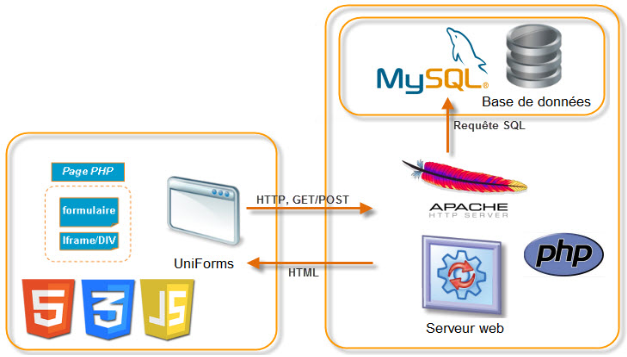
\includegraphics [width=90mm]{images/architecture.png}}
\end{center}
\caption{Fonctionnement de l'application}\label{fonctionnementAppli}
\end{figure}

\subsection{Base de données}\label{sec:BDD}
La figure~\ref{schemaBDD} montre la structure de la base de données. Elle est faite de telle manière à ce que chaque groupe d'éléments de formulaire puisse être répondu par un utilisateur. Un ensemble de groupe forme un formulaire.\\
Pour chaque élément, il peut y avoir une (champs d'entrée à une réponse) ou plusieurs (cases à cocher) réponses.\\
Les mêmes champs peuvent être renseigner pour tous les types d'éléments (table ``formelement''), si jamais l'élément à plusieurs options (cases à cocher ou boutons radios), la table ``elementoption'' se remplira avec toutes les options.\\
Pour stocker l'état d'une réponse, dans la table ``answer'' la valeur de ``answer\_status'' est ``0'' pour enregistré, ``1'' pour envoyé. De même pour ``form\_status'' pour le formulaire enregistré et publié, les valeurs sont respectivement ``0'', ``1''.\\ 
Si l'on souhaite ajouter un nouveau type d'élément, la base de données n'a pas besoin d'être modifiée. En effet, chaque élément proposé sur la page de création de formulaire correspont à un nombre. Ce nombre est le type\_element de la classe ``formelement''. Pour ajouter un nouveau type d'élément, il suffit de définir un nombre pour ce nouveau type. En effet, que l'élément possède une ou plusieurs valeurs, lors de l'enregistrement du formulaire, l'élément s'enregistrera dans la base de données comme n'importe quel autre, sauf que son type\_element sera le nouveau défini.\\
Chaque formulaire peut être répondu une ou plusieurs fois par le même destinataire. Cette information est stockée avec l'attribut ``group\_limit'' de ``formgroup''. En effet, répondre à un formulaire correspond à répondre à un ou plusieurs groupes d'éléments.\\
``elementanswer'' est une table de jointure entre ``answer'', ``answervalue'' (qui contient la ou les valeurs de réponses) et ``formelement''.

\begin{figure*}
\begin{center}
\makebox[\linewidth]{%        to center the image
  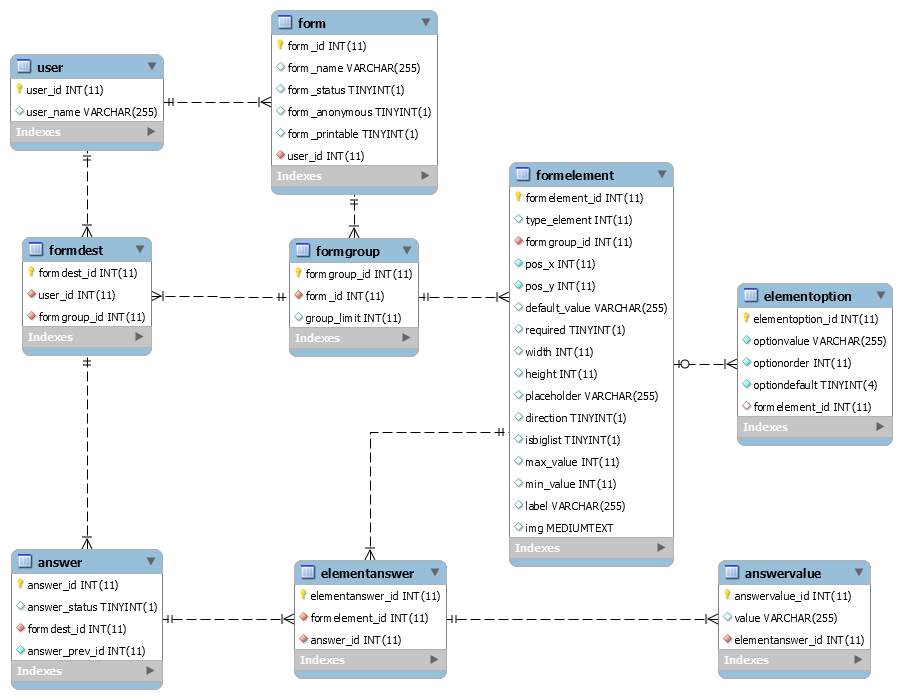
\includegraphics [width=150mm]{images/bdd_diagram.png}}
\end{center}
\caption{Schéma de la base de données}\label{schemaBDD}
\end{figure*}

\subsection{Classes PHP}
Afin d'extraire et de remplir des informations dans les tables de la base de données figure~\ref{schemaBDD}, des classes PHP ont été utilisées.\\
On remarque figure~\ref{diagrammeClasses} que les classes construites sont plus ou moins les mêmes que les tables de la base de données. On retrouve ``Form'' pour ``form'' de la base de données, ``Group'' pour ``formgroup'', ``User'' pour ``user'', ``Element'' pour ``formelement'' et ``elementoption'' et enfin ``Answer'' pour ``answer'', ``elementanswer'' et ``answervalue''.\\
Cette structure nous permet en créant des objets d'extraire et remplir facilement les données des tables de la base de données et de les exploiter dans notre application.

\begin{figure*}
\begin{center}
\makebox[\linewidth]{%        to center the image
  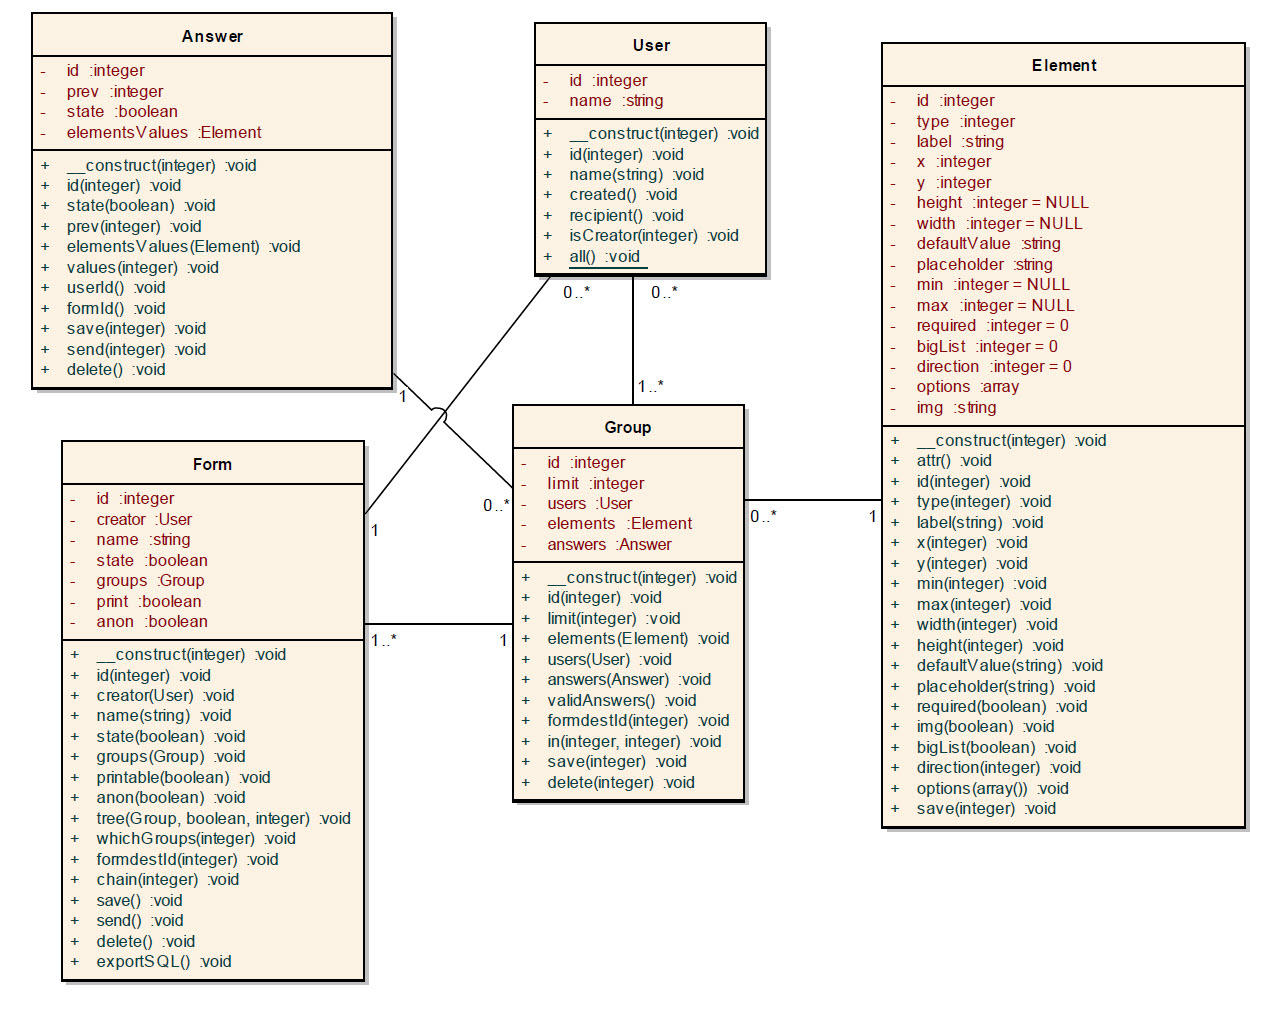
\includegraphics [width=160mm]{images/class_diagram.jpg}}
\end{center}
\caption{Diagramme de classes}\label{diagrammeClasses}
\end{figure*}

\section{Connexion}
L’ensemble des utilisateurs ayant un compte CAS à l’Université de Nice peuvent utiliser UniForms, et ce sans avoir besoin de se créer un compte au préalable. Comme déjà précisé, il est également possible d’accéder à l’application sans s’authentifier, dans le cadre de la réponse à un formulaire anonyme.\\

Le service CAS est un système d’authentification unique sur un ensemble de site web. C’est le système utilisé dans la majorité des Université de France et est très répandu dans les Universités à travers le monde.\\
Un serveur CAS étant déjà en place à l’université, nous avons uniquement eu besoin d’implémenter un client CAS pour notre application. CAS gère l’authentification d’une personne à l’aide d’un cookie stocké dans le navigateur de l’utilisateur et de tickets échangés entre l’application cliente et le serveur.\\
Nous proposons donc à nos utilisateurs n’ayant pas un cookie à jour de se connecter à travers le portail de connexion usuel de l’Université. Lorsque le serveur CAS nous retourne un identifiant, ils sont ensuite redirigés vers notre page d’accueil. Nous proposons de même un lien vers la page de déconnexion usuelle de l’Université pour libérer son cookie, bien que se scénario ne se présente pas souvent dans la pratique.

%---------------------------------Section fonctionnalité développées----------------
\section{Les fonctionnalités développées}
\subsection{Création/Modification de formulaire}
\subsubsection{Éléments choisis (lesquels/pourquoi)}
Douze éléments sont proposés. Ils ont été choisis de manière stratégique afin de proposer un ensemble assez divers, que l’utilisateur puisse exprimer ce qu’il souhaite tout en prenant en compte les contraintes de temps qui nous étaient imposées pour la réalisation du projet.\\
Trois types d'éléments sont donc proposés :
\begin{description}
\item [Pour des questions ouvertes] : Champs d'entrée texte simple, date, heure, paragraphe, téléphone et nombre.
\item [Pour des questions fermées] : Cases à cocher et boutons radio.
\item [Pour la mise en page] : Label, carré (ou rectangle si modification de la taille), cercle (ou rectangle arrondi si modification de la taille) et insertion d'images.
\end{description}
Ainsi l’utilisateur peut proposer tous les types de questions : questions ouvertes de type texte (champs texte court ou long), questions ouvertes de type prédéfini (heure, date, téléphone), questions à choix unique (boutons radios) et questions à choix multiple (cases à cocher).\\
Certains éléments n'ont pas été implémentés, par exemple le champs d'entrée URL car nous avons pensé qu'ils n'étaient pas indispensables. En effet, si l'utilisateur souhaite que le destinataire entre une URL par exemple, l'élément pour proposer ce type de champs d'entrée n'est pas disponible, cependant un alternative est possible, l'utilisateur peut proposer un champs texte qui peut être rempli par un URL. De plus, pour implémenter un nouvel élément, il suffit de l'ajouter dans la liste des éléments de la page createform.php et la gérer dans drag.js, ensuite il n'y a aucun besoin de modifier la base de données comme expliqué section~\ref{sec:BDD} et les classes PHP n'ont nul besoin d'être modifiées.

\subsubsection{Groupes}
L'idée de départ était d'offrir la possibilité à l'utilisateur de créer des formulaires pouvant être remplissable par partie par différents utilisateurs.\\
Deux solutions nous paraissaient faisables. La première consistait à glisser-déposer des groupes sur le champs quadrillé puis d'insérer les éléments dans les groupes sur la zone de drop. La deuxième consistait à créer un formulaire normalement puis créer des groupes sur une autre zone avec la possibilité d'en faire ou pas. Les éléments n'étant dans aucun groupe aurait un destinataire commun.\\
Nous avons penché pour la deuxième solution car la première avait deux points négatifs. Premièrement, les éléments devaient forcément se positionner sur la même zone pour être regroupés et donc enlevait de la liberté de création et deuxièmement parce que demander à l'utilisateur les destinataires et nombre maximal de remplissage dans ce cas était moins clair pour l'utilisateur. Alors que la deuxième solution propose une zone spécialement dédiée aux groupes et donc l'utilisateur dispose d'une vue d'ensemble sur ces derniers.\\
Un autre problème s'est posé, celui des éléments restants, en effet, si l'utilisateur ne souhaite pas faire de groupe, il devait tous les mettre dans un groupe avec le destinataire. C'est pourquoi nous avons décidé de créer un groupe par défaut, le premier affiché non supprimable, il contient par défaut tous les éléments restants. Ainsi, l'utilisateur renseigne les paramètres destinataires et nombre maximum de réponse de ce groupe pour un formulaire à un seul destinataire.\\
Cette manière de faire permet d'envoyer des formulaires pour plusieurs destinataires remplissable plusieurs fois, le nombre de réponse attendu est donc de l'ordre du nombre de destinataires du premier groupe multiplié par le nombre de destinataires du deuxième groupe jusqu'au dernier groupe et multiplié par le nombre de réponse possible de chaque groupe.

\subsubsection{Destinataires}
Pour la sélection de destinataires, un champs d’entrée est proposé. Dans ce champs à chaque entrée de caractère, des propositions de destinataires sont affichées.\\
Ce choix pour la sélection de destinataires a été fait pour palier au grand nombre de destinataires qui seront disponibles. En effet, ce nombre peut atteindre deux ou trois milles, l’affichage de tous les destinataires sur une page n’étaient donc pas adapté.\\
D’autre part, la sélection de destinataire se fait par identifiant CAS, c’est-à- dire que le créateur doit connaître les identifiants des personnes à qui il souhaite envoyer le formulaire. Ce choix est dû au fait que les informations des utilisateurs noms, prénoms, promotion,...se situe sur LDAP et nous n'avons pas eu les droits d'accès. Avec les droits d'accès, nous aurions pu proposer d'autres solutions de sélection de destinataire par groupe, promotion, recherche par nom puis prénom,...

\subsubsection{Paramètres}\label{sec:parametres}% (lesquels et pourquoi avoir choisi ces paramètres)
Deux paramètres nous ont paru indispensables et suffisants. %
\begin{itemize}
\item “Imprimable” car dans les objectifs du DoW mais pas forcément obligatoire pour chaque formulaire.
\item “Anonyme” pour pouvoir offrir la possibilité de faire un sondage comme les concurrents sans connaître l’identité des personnes et donc soumettre un formulaire à des personnes externes à l’université.
\end{itemize}
Ces paramètres sont ensuite traités en PHP et sauvegardé dans la table ``form'' de la base de données, voir section~\ref{schemaBDD}.\\

D'autres paramètres pour insérer un thème au formulaire ou choisir les dimensions de la feuille du formulaire aurait pu être ajouté cependant, les objectifs étaient clairs et précis, nous n'avons pas voulu en ajouter trop car le temps était limité. Si nous avions implémenté d'autres paramètres, il aurait juste fallu ajouter les champs correspondant dans la base de données et les méthodes pour remplir les informations dans la base.

\subsubsection{Glisser-déposer}
Un glisser-déposer aussi appelé drag'n'drop a été implémenté en JQuery afin de donner la possibilité de créer le formulaire le plus proche possible de la réalité. Le champs disponible pour la position des éléments est de la taille d’une page A4 et est quadrillée pour l'aide au positionnement, une fois rempli la page s’agrandit d’une page en hauteur.\\
L'ensemble des éléments positionnés est au fur et à mesure enregistré grâce à des objets JavaScript. Dans chaque objet (correspondant à un élément), les paramètres sont enregistrés en tant qu'attribut de l'objet. On peut ainsi récupérer les paramètres que l'utilisateur renseigne à chaque fois qu'il en selectionne un, et remplir les champs de paramètre. L'utilisateur peut alors modifier les paramètres de l'éléments.\\
Lors de l'enregistrement (ou publication) du formulaire, la liste de tous les objets des éléments est envoyé en JSON\footnote{JavaScript Object Notation} par l'intermédiaire d'un champs d'entré ``input'' caché à la page add\_form.php qui traite tous les éléments avec leurs paramètres pour créer les objets PHP et insérer toutes les informations dans la base de données vu section~\ref{sec:BDD}.\\

Pour la formation de groupes, c’est le même principe, sauf que les informations des groupes ne sont récupérées qu’à la fin, au moment de l’enregistrement (ou validation) car le paramètre destinataire est conservé par une autre variable USERSGROUP de createform et le nombre maximum de réponse autorisé est conservé par les champs nombres de chaque groupe.\\
Au moment de l'enregistrement (ou de la publication), on vérifie que chaque groupe à bien un destinataire, si ce n'est pas le cas, un message d'alerte est affiché à l'utilisateur.

\subsection{Répondre à un formulaire} 
Pour répondre à un formulaire, comme annoncé dans les scénarios section~\ref{sec:scenarios}, il est possible de le faire de manière papier ou par l'intermédiaire de l'application. Ce choix est dû au fait que l'application devait remplir les besoin de création de formulaire de manière classique mais aussi les e-formulaires du web pour obtenir les résultats numériquement pour une traitement plus simple et court.\\
Sur le web, la page de formulaire est présenté aux destinataires telles qu'elle a été créée. Sur papier, c'est la même chose sauf que les réponses ne sont pas enregistrées dans la base de données.

\subsection{Consulter les réponses aux formulaires}
\subsubsection{En ligne}
La consultation en ligne est la même que si l'utilisateur consultait les réponses sur papier car les réponses sont présentées tel que le formulaire a été rempli à l'utilisateur et il peut passer de résultat en résultat par deux boutons ``Next'' et ``Back''.

\subsubsection{Télécharger les résultats}
Deux formats de téléchargement des résultats sont proposés, SQL et CSV.\\
Ces choix de format ont été faits suivant le type des futurs utilisateurs de notre application.\\
CSV est utile pour les utilisateurs se servant d'un tableur (par exemple Excel un logiciel appartenant au pack Office installé dans la plupart des entreprises et donc à l'université ou LibreOffice Calc, OpenOffice,...). Une fois importé dans Excel, cela permet une manipulation des données par l'utilisateur de manière aisée sans avoir besoin de connaissances informatiques spécifiques.\\
SQL est pour une manipulation plus complexe des données, mais peut être utile si les données doivent être exporté dans une nouvelle base et/ou utilisé dans une autre application. Les utilisateurs visés sont ceux connaissant le langage SQL.\\
Il ne nous a pas paru necessaire d'autres formes d'exportation, en effet, l'exportation dans une page web existante peut être réalisé avec l'exportation SQL et le xls avec le CSV. Beaucoup de cas découlent de ces deux formats.

%---------------------------Section Validation
\section{Validation}
Lorsque l'application est réalisé, il convient que notre encadrant s'assure qu'il répond aux objectifs cités dans le Description Of Work, pour cela nous avons programmé des réunions après la fin de chaque lot dans le but d’assurer le bon avancement du projet en fonction des objectifs attendues.

\subsection{Outils de tests utilisés}
Afin de réaliser les tests nous avons utiliser deux outils, SimpleTest pour les tests des classes PHP et Sélénium IDE pour les tests de scénarios.\\
Bien que PHPUnit soit un standard des framework de tests PHP, nous avons choisi SimpleTest car il possède une interface web pour l’exécution des tests. De plus, l’équipe travaillant sur deux systèmes d’exploitation différents, SimpleTest fonctionnait sur les deux à la différence de PHPUnit.\\
Selenium est un plugin fonctionnant sur de nombreux navigateurs (Firefox, Chrome, Opéra,...) permet de tester les scénarios.

\subsection{Tests classes PHP} %TODO
Afin de vérifier le bon fonctionnement des méthodes de nos classes PHP, nous les avons testé en utilisant SimpleTest.

\subsection{Tests scénarios} %TODO
Sélénium IDE pour les tests d’interface

\subsection{Tests utilisateurs}
Nous avons essayé de faire appel à des personnes de l’université qui n’ont jamais entendu parlé de ce projet, leurs réactions ne seront donc pas influencées et nous pourront noter les facilités et/ou difficultés rencontrées et ainsi améliorer l’utilisabilité. Malheureusement nous n’avons pas pu le faire pour la simple raison que les créneaux consacrés pour le projet de fin d'étude en temps complet coïncident avec les vacances universitaires, c’est pourquoi il a été difficile pour nous et pour notre encadrant pour trouver des personnes disponibles.

%------------------------------Section Positionnement
\section{Positionnement}
Ici, nous allons positionner notre application par rapport à l’état de l’art. Tout d’abord nous allons la confronter aux logiciels classiques puis aux e-formulaires existants du web.
\subsection{Face aux logiciels classiques}
Dans l’état de l’art nous avions étudié trois logiciels,  Microsoft Office\cite{urlMicrosoft} (Word et Excel), Adobe\cite{urlAdobe} (PDF LiveCycle Designer) et Latex.\\
Le défaut commun à ces trois logiciels étaient qu’ils demandaient tous un minimum de connaissances informatiques.\\
Notre application se démarque de ces dernières car permet de réaliser la même chose que ces logiciels mais sans avoir besoin nécessairement de connaissances informatiques. Uniforms propose une interface graphique pour tout, de la création des formulaires à la consultation des réponses en passant pas la réalisation des réponses et n’a pas besoin d’écrire de code.
Un autre défaut majeur est que les logiciels Microsoft Office et Adobe sont payants et accessibles par le système d’exploitation Windows uniquement, ce qui restreint le nombre d’utilisateur potentiel et dans l’autre sens également, les personnes souhaitant créer des formulaires n’ont pas tous accès à ces outils. En revanche, notre application web est accessible depuis n’importe quel système d’exploitation et est totalement gratuite.
De plus, certain outil tel que Word ne propose pas une variété d’éléments suffisants, seulement des champs de texte simple, pas de spécification pour un champ de date, d’heure ou de numéro de téléphone…\\
Uniforms a été développée de manière à proposer à l’utilisateur un outil accessible à tous sans les inconvénients cités précédemment.

\subsection{Face aux e-formulaire}
De nombreux e-Formulaires sur le web proposent des interfaces graphiques pour réaliser des formulaires. Tous proposent des interfaces plus ou moins intuitives, l’utilisateur n’a pas besoin d’écrire de code. \\
Ici, nous allons comparer ces applications à Uniforms sous divers points de vue.
\subsubsection{Utilisabilité}
Les applications existantes n’obligent pas forcément l’utilisateur à se connecter, c’est pourquoi, il doit créer le formulaire en une fois, sans pause ni coupure de connexion. Pour un meilleur confort de l’utilisateur, nous avons pensé à implémenter la fonctionnalité d’enregistrement pour modification et validation plus tard tout autant dans la création de formulaires comme dans les réponses faites par les destinataires.\\
Pour une meilleure efficience, nous avons également pensé à proposer un système de placement des éléments sur la page là où l’utilisateur le souhaite, c’est-à-dire que le créateur dispose d’un glisser-déposer là où il le souhaite sur la page et non les disposer les uns sous les autres de manière verticale comme le propose WebQuest par exemple. Également, l’utilisateur n’est pas obligé de placer des groupes de une question et un champs de réponse comme bons nombres des applications existantes. Cela laisse la liberté de création à l’utilisateur.\\
Au niveau de l’efficacité, elle est comparable aux applications existantes car le système est similaire, glisser-déposer d’éléments sur la page et renseignement des propriétés des éléments (requis, taille,...).\\
Les applications existantes proposent une version mobile, notre application est réalisée avec Bootstrap, donc responsive, mais la page de création devant être imprimable a donc une taille de page A4, il n’est donc pas possible de créer un formulaire sur un mobile, mais la consultation, téléchargement des résultats est possible. Pour ce point, les applications existantes surpassent notre application.\\
Pour ce qui est de l’interface, elle est simple, intuitive et un manuel d’utilisation a été rédigé afin d’en faciliter l’utilisation tout comme pour les application existantes.
\subsubsection{Éléments proposés}
Les éléments proposés dans notre application sont au nombre de douze (label, nombre, champs texte, paragraphe, boutons radios, cases à cocher, date, heure, numéro de téléphone, image, carré et cercle). D’autres application telles que Oxiform\cite{urlOxiForm} ou Typeform\cite{urlTypeForm} en propose plus en y ajoutant le champs d’url, d’email, de liste déroulante...à ceux que nous proposons.\\ Cependant, notre application n’est pas totalement mal placé car certaines applications proposent moins d’éléments, WebQuest n’en propose que huit.
\subsubsection{Anonymat}\label{sec:anonymat}
La question de l’anonymat à la réponse d’un formulaire se pose très souvent. Les destinataires doivent-ils être identifié ou non ? L’entrée de leurs identifiants (nom, prénom, numéro,...) est-elle suffisante pour que le créateur soit sur que la réponse a été effectuée par un certain destinataire.\\
Sur le web, la majorité des applications de création de formulaire ne propose pas d’identification, n’importe quelle personne étant en possession du lien du formulaire peut y répondre. Par exemple, Oxiform ou Typeform. \\
Nous avons voulu y rémédier, notre application propose de créer des formulaires anonymes ou non, ce qui permet de faire des sondages sans se soucier de qui répond au formulaire tout comme les applications déjà existantes, mais aussi de créer des formulaires nominatifs, ajouter des destinataires précis grâce au système d’identification CAS intégré.
\subsubsection{Remplir un formulaire à plusieurs}
Une des fonctionnalités majeures de notre application est le fait de pouvoir déterminer des utilisateurs pour certains champs d'entrées. Le formulaire peut alors être rempli à plusieurs.\\
Dans nos recherches, nous n'avons pas trouvé de concurrent à ce niveau là, car comme dit à la section~\ref{sec:anonymat} la plupart des applications de formulaires existants proposent des formulaires anonymes avec aucun moyen de définir plusieurs destinataires pour un seul et même formulaire.
\subsubsection{Confidentialité}
Toutes les applications du web stockent les données dans le Cloud, ce qui veut dire que les applications existantes disposent d’autant de données que de champs de formulaire remplis par les destinataires. Pour ce point là, Uniforms a pour principal but de se mettre au service de l’université, il y est hébergé, les données ne sont donc pas partagées avec un tiers.
\subsubsection{Design}
Des applications telles que Oxiform ou Typeform proposent des thèmes. Notre application n’a pas pour cet objectif, mais plutôt celui de rendre le formulaire imprimable, le thème “noir sur blanc” est donc tout à fait justifié.
\subsubsection{Exportation}
Diverses méthodes d’exportation sont disponibles avec les applications existantes, xml, csv, xls pour FormPro\cite{urlFormPro}, intégration à une page web existante pour Oxiform. Notre application ne propose que l’exportation en csv, sql et la consultation des résultats en ligne. Les résultats sont exportables par moins de moyens et aucune option de statistiques sur résultats n’est possible à la différence de FormPro.
\subsubsection{Gratuité}
Notre application est totalement gratuite, toutes les applications existantes auxquelles nous avons comparé uniforms précédemment sont soit limités en nombre de formulaire ou dans le temps (sauf Google Form\cite{urlGoogleForm}).
\subsection{Synthèse}
Nous avons précédemment comparé notre application à celles existantes sous divers aspects.\\ En général, nous avons vu que notre application se démarquait pour certains aspects comme la confidentialité, l’anonymat ou même la gratuité qui sont des points très important. Mais surtout sur le fait qu'un formulaire peut être rempli par plusieurs personnes ce qui n'a pas été trouvé dans une autre application.\\
En revanche, sous d’autres aspects moins important, elle est plus faible, par exemple le nombre d’éléments disponibles qui, en moyenne, est plus élevé. L’exportation de données ne se fait que sous deux formes alors que d’autres applications proposent beaucoup plus. Cependant, l’objectif de notre application n’est pas l’exportation, mais plutôt de pouvoir gérer les résultats en dehors de l’application pour des utilisateurs de l'université, c'est-à-dire utilisant un tableaur et/ou SQL. L’objectif est donc atteint. \\
Au niveau du design, notre application a pour but d’être imprimable, il est donc normal de ne pas proposer de thèmes comme les applications existantes. Cependant, il suffirait d'ajouter un paramètre pour le thème et des paramètres de coloration des éléments pour obtenir quelque chose de similaire comme expliqué section~\ref{sec:parametres}.\\
En ce qui concerne l’utilisabilité un point très important suivant notre DoW, elle se positionne au même niveau que les applications existantes, ergonome et intuitive malgré le fait qu’elle ne propose pas de version mobile, elle propose néanmoins des fonctionnalités compensant cette faiblesse, par exemple la modification (formulaire ou réponse).\\
Pour présenter une version mobile, il suffirait d'ajouter un paramètre pour les dimensions de la page de formulaire comme expliqué en section~\ref{sec:parametres}, ainsi, l'utilisateur pourra créer un formulaire pour mobile depuis un mobile car le framework Bootstrap se charge du responsive design.

%--------------------------Section Conclusion
\section{Conclusion}
\subsection{Résultats obtenus}
Au début du projet, cinq critères de succès ont été définis et six objectifs ont été fixés.\\ 
Nous allons ici voir ce qui a été réalisé. 
\subsubsection{Objectifs}
\begin{itemize}
\item Uniformiser la représentation d'un formulaire\\
L’application propose bien une représentation imprimable proche de celle réalisée par l’utilisateur.
\item Présenter une interface utilisateur ergonomique\\
C’est un des points les plus importants pour notre application, la facilité d’utilisation pour un non informaticien, une interface intuitive. Notre tuteur qui a également le rôle de client nous a conseillé pour le développement de l’interface et a confirmé son utilisabilité. Ce point est donc validé et valide également un critère de succès.
\item Garantir la confidentialité des données\\
L’authentification CAS permet de nominer les créateurs et les destinataires. De plus, l’application étant hébergée à l’université, cela permet de ne pas avoir à partager les données avec un tier. Ce point valide également un critère de succès.
\item Permettre la gestion de collections de formulaires\\
Uniforms permet la gestion des formulaires créés et des formulaires reçus, avec les quatre opérations CRUD\footnote{Create Read Update Delete}, création, lecture, mise à jour et suppression.
\item Donner la possibilité de pré-remplir des champs\\
Ce point là a été abandonné en cours de projet, car la fonctionnalité de création de formulaire dit “Collaboratif” a dû être revu et son temps de développement a augmenté pour prendre en compte certains éléments importants (ordre de remplissage, nombre de réponses autorisée,...). Avec accord du client, nous avons décidé de développer le formulaire “collaboratif” et d’abandonner le pré-remplissage.
\item Livrer une documentation\\
Deux documentations ont été réalisées. Une documentation technique à l’aide de PHPdoc pour les éventuels futurs développeurs qui souhaiteraient reprendre le projet et un manuel utilisateur afin d’expliquer en détail le fonctionnement de l’application aux utilisateurs.\\
Cette documentation valide également un critère de succès.
\end{itemize}

Les autres critères de succès, génération de formulaire papier exploitable et création d’un package sont également validés car lors de la création d’un formulaire, l’utilisateur peut imprimer son formulaire grâce à la combinaison de touche Ctrl + P. Il peut ainsi vérifier sa mise en page finale.\\
Pour le package d’installation, seul l'installation de la base de données est nécessaire, c'est pourquoi nous proposons une page où les informations de la base de données sont requies et un script l'installe.

\subsubsection{Synthèse}
Pour conclure sur les résultats obtenus, nous pouvons dire que tous les critères de succès ont été atteints. Hormis l’objectif du pré-remplissage des champs qui est compensé par le formulaire “collaboratif”, tous les objectifs ont également été atteints.

\subsection{Perspectives}
À la vue de nos résultats et de l’état de l’art, on pourrait imaginer diverses améliorations.\\
Premièrement, au niveau des utilisateurs. Actuellement, les utilisateurs autorisés sont ceux pouvant s’identifier avec CAS. Il pourrait être intéressant d’ouvrir le champs des utilisateurs à des personnes externes à l’université. Par exemple, si l’on souhaite recueillir l'opinion de personne ayant assistée un événement de l’université. Un compte temporaire serait créé pour qu’ils répondent au formulaire. À la différence d’un formulaire anonyme, les personnes qui répondront seront définies.\\
Deuxièmement, la liste des éléments disponibles est limitées, proposer plus d’éléments comme un champs d’url, d'adresse mail, liste déroulante... \\
Troisièmement, les champs de réponses sont vides lorsqu’ils sont proposés au destinataire, il serait pertinent de développer la fonctionnalité d’auto-remplissage par bases de données externes. Par exemple, si le créateur possède en local une base de données concernant les promotions de chaque élève, qu’il puisse, par l’intermédiaire d’un script qu’il écrira, remplir les champs de promotion de élève du formulaire soumis.




\appendix
%\section{Appendix Title}

%This is the text of the appendix, if you need one.

%\acks

%Acknowledgments, if needed.

% We recommend abbrvnat bibliography style.

\bibliographystyle{abbrvnat}

% The bibliography should be embedded for final submission.

\begin{thebibliography}{}
\softraggedright
\bibitem{urlPHP} Site web PHP : \url{http://php.net/}
\bibitem{urlMySQL} Site web MySQL : \url{http://www.mysql.fr/}
\bibitem{urljQuery} Site web jQuery : \url{http://jquery.com/}
\bibitem{urlBootstrap} Site web Bootstrap : \url{http://getbootstrap.com/}
\bibitem{urlOxiForm} Site web OxiForm : \url{http://www.oxemis.com/solution-logiciel-formulaires-oxiforms.php}
\bibitem{urlTypeForm} Site web TypeForm : \url{http://www.typeform.com/}
\bibitem{urlGoogleForm} Site web GoogleForm : \url{http://www.google.com/forms/about/}
\bibitem{urlMicrosoft} Site web Microsoft Office : \url{http://office.microsoft.com/fr-fr/}
\bibitem{urlAdobe} Site web TypeForm : \url{http:// www.adobe.com/products/server/adobedesigner}
\bibitem{urlWebQuest} Site web WebQuest : \url{http://www.webquest.fr/}
\bibitem{urlFormPro} Site web FormPro : \url{https://fr.formpro.com/}

\end{thebibliography}


\end{document}

%                       Revision History
%                       -------- -------
%  Date         Person  Ver.    Change
%  ----         ------  ----    ------

%  2013.06.29   TU      0.1--4  comments on permission/copyright notices

